\documentclass[fontset=windows]{ctexart}
\usepackage{fancyhdr}
\usepackage{xcolor}
\usepackage{listings}
\usepackage{geometry}
\usepackage{graphicx}
\usepackage{multirow}

\geometry{a4paper, left=2.5cm, right=2.5cm, top=3cm, bottom=3cm}

% 设置页眉
\pagestyle{fancy}
\fancyhf{}
\fancyhead[L]{AIGC 创新赛}  % 左侧显示章节标题
\fancyhead[R]{FuFu.AI}  % 右侧自定义文字
\renewcommand{\headrulewidth}{0.4pt}

% 定义代码块样式
\lstset{
    backgroundcolor=\color{gray!10},
    basicstyle=\small\ttfamily,
    frame=single,
    numbers=left,
    numberstyle=\tiny\color{gray},
    breaklines=true,
    tabsize=4
}

\begin{document}

% 独立标题页
\begin{titlepage}
    \thispagestyle{empty}
    \vspace*{1cm}
    \centering
    \begin{figure}[h]
        \small
        \centering
        
\includegraphics[width=0.4\textwidth]{./figure/LOGO.png}
    \end{figure}
    \vspace*{1cm}
    {\LARGE\bfseries IA Calendar 技术文档 \\[1.5em]}
    {\large Team: FuFu.AI \\[2em]}
    \vspace{1cm}
    {\normalsize
        \begin{tabular}{@{}ll@{}}
            上官子涵 & 西北工业大学 \\
            钟习伟  & 湖南大学   \\
            吴思贤  & 华南理工大学 \\
            何泓儒  & 华南理工大学 \\
            杨锦龙  & 华南理工大学 \\[2cm]
        \end{tabular}}

    \vfill
\end{titlepage}

% 重置页面样式
\clearpage
\pagestyle{fancy}
\setcounter{page}{1}

\vspace{2cm}

\section{应用架构}
\subsection{整体架构}

\begin{figure}[h]
    \small
    \centering
    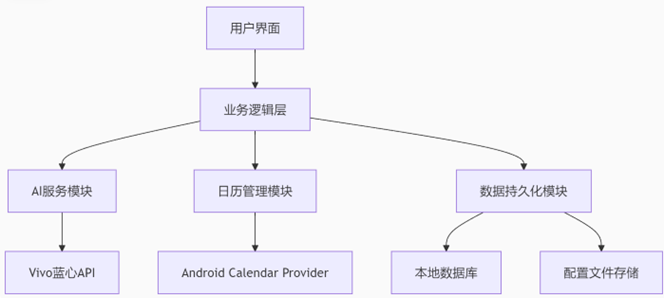
\includegraphics[width=12cm]{figure/structure.png}
    \caption{应用架构示意图} \label{fig:aa}
\end{figure}

\subsection{模块职责说明}
\begin{table}[h!]
    \centering
    \caption{模块职责}
    \begin{tabular}{ccc}
        \hline
        模块                  & 组件                 & 功能描述                  \\ \hline
        \multirow{2}*{交互层}  & ChatActivity       & 实现多轮对话、消息渲染与用户输入处理    \\
        ~                   & ScheduleConfigView & 显示AI生成的日程配置详情         \\
        AI服务                & VivoGPTClient      & 封装API请求签名、参数构造、响应内容解析 \\
        \multirow{2}*{日历管理} & CalendarWriter     & 处理日历事件创建/修改/删除        \\
        ~                   & CalendarReader     & 在指定筛选条件下读取用户近期日程      \\
        \multirow{2}*{数据层}  & SharedPrefManager  & 存储用户偏好设置、会话上下文        \\
        ~                   & RoomDataBase       & 持久化存储历史配置             \\
        \hline
    \end{tabular}
\end{table}

\newpage{}
\section{核心功能实现}

\begin{lstlisting}[language=Java, caption=数据模型定义]
public class ScheduleConfig {
    public List<ScheduleEvent> events = new ArrayList<>();
    public String analysis; // AI分析建议

    // 添加事件
    public void addEvent(ScheduleEvent event) {
        events.add(event);
    }
}

// 日程事件类
public class ScheduleEvent {
    public String eventId;    // 事件唯一ID
    public String title;      // 事件标题
    public Date startTime;    // 开始时间
    public Date endTime;      // 结束时间
    public List<Integer> reminders = new ArrayList<>(); // 提醒时间(分钟)
    public String location;   // 事件地点
}
\end{lstlisting}

当处理用户自然语言输入时,首先通过DialogManager的状态机控制对话流程。在SCHEDULING状态下,用户输入经VivoGPTClient传输至云端AI,其响应数据通过ScheduleParser进行结构化转换。
当收到VivoGPT的JSON响应时,ScheduleParser按以下顺序处理:

\begin{itemize}
    \item 创建空配置对象
    \item 解析顶层analysis字段
    \item 遍历events数组:
    \item 1) 转换时间字符串为Date对象
    \item 2) 处理时区标识
    \item 3) 收集提醒设置到整数列表
\end{itemize}

\begin{lstlisting}[language=Java, caption=AI响应解析器]
public class ScheduleParser {
    private static final String TAG = "ScheduleParser";
    private static final SimpleDateFormat DATE_FORMAT = 
        new SimpleDateFormat("yyyy-MM-dd'T'HH:mm:ssZ", Locale.CHINA);

    // 解析AI返回的JSON数据
    public ScheduleConfig parseAIResponse(String jsonResponse) {
        ScheduleConfig config = new ScheduleConfig();
        try {
            JSONObject root = new JSONObject(jsonResponse);
            config.analysis = root.optString("analysis", "无建议");

            // 解析事件列表
            JSONArray events = root.getJSONArray("events");
            for (int i = 0; i < events.length(); i++) {
                JSONObject eventJson = events.getJSONObject(i);
                ScheduleEvent event = new ScheduleEvent();
                event.eventId = eventJson.getString("id");
                event.title = eventJson.getString("title");
                event.startTime = parseDate(eventJson.getString("start_time"));
                event.endTime = parseDate(eventJson.getString("end_time"));
                
                // 解析提醒设置
                JSONArray reminders = eventJson.getJSONArray("reminders");
                for (int j = 0; j < reminders.length(); j++) {
                    event.reminders.add(reminders.getInt(j));
                }
                
                config.addEvent(event);
            }
        } catch (JSONException | ParseException e) {
            Log.e(TAG, "解析失败: " + e.getMessage());
        }
        return config;
    }

    // 日期解析工具方法
    private Date parseDate(String dateStr) throws ParseException {
        return DATE_FORMAT.parse(dateStr.replace("Z", "+0800")); // 处理时区
    }
}

\end{lstlisting}

\begin{lstlisting}[language=Java, caption=多轮对话管理]
public class DialogManager {
    private enum State { IDLE, SCHEDULING, CONFIRMING }
    private State currentState = State.IDLE;
    private ScheduleConfig draftConfig;

    // 处理用户输入
    public void handleInput(String userInput) {
        switch (currentState) {
            case IDLE:
                if (userInput.contains("安排日程")) {
                    currentState = State.SCHEDULING;
                    draftConfig = new ScheduleConfig();
                    promptAI("请描述您的日程需求");
                }
                break;
                
            case SCHEDULING:
                if (userInput.contains("确认")) {
                    currentState = State.CONFIRMING;
                    showPreview(draftConfig);
                } else {
                    processSchedulingStep(userInput);
                }
                break;
        }
    }

    private void processSchedulingStep(String input) {
        // 调用AI接口获取初步配置
        String aiResponse = callVivoAPI(input);
        ScheduleConfig partialConfig = new ScheduleParser().parseAIResponse(aiResponse);
        
        // 合并到草稿配置
        draftConfig.events.addAll(partialConfig.events);
        draftConfig.analysis = partialConfig.analysis;
    }
}
\end{lstlisting}

\newpage{}
\section{AI Prompt}
在调用API的Java程序中,指定\(Header\)中的\(Content-Type\)为\(JSON\),以便于输出的标准格式化,其提示词如下所示:
\begin{lstlisting}[caption=日程生成Prompt]
你是一个专业的时间管理助手,请按以下规则处理用户输入:
1. 识别时间要素(日期、时间、周期)
2. 分解复杂任务为可执行事项
3. 输出JSON格式
{
  "events": [
    {
      "title": "事件标题",
      "start_time": "YYYY-MM-DD HH:mm",
      "end_time": "YYYY-MM-DD HH:mm",
      "reminder": 15 // 提前提醒分钟数
    }
  ],
  "analysis": "时间安排合理性分析"
}
\end{lstlisting}
\begin{lstlisting}[language=Java, caption=日程分析Prompt]
请根据以下用户日程进行分析:
1. 识别时间冲突
2. 建议优化方案
3. 生成改善建议的日程
输出格式:
{
  "analysis": "总体分析",
  "suggestions": [
    {
      "type": "time_conflict|overload|inefficient",
      "description": "问题描述",
      "recommendation": "调整建议"
    }
  ],
  "new_events": [...] // 建议新增的日程
}
\end{lstlisting}

\newpage{}
\section{所需权限与配置}
\begin{lstlisting}[language=Java, caption=日历读取相关权限]
<uses-permission android:name="android.permission.READ_CALENDAR"/>
<uses-permission android:name="android.permission.WRITE_CALENDAR"/>
\end{lstlisting}
\begin{lstlisting}[language=Java, caption=API调用相关参数]
private static final String APP_ID = USER_ID;
private static final String APP_KEY = USER_KEY;
private static final String API_URL = "https://api-ai.vivo.com.cn/vivogpt/completions";
\end{lstlisting}

\newpage{}
\section{预期流程}
\begin{figure}[h]
    \small
    \centering
    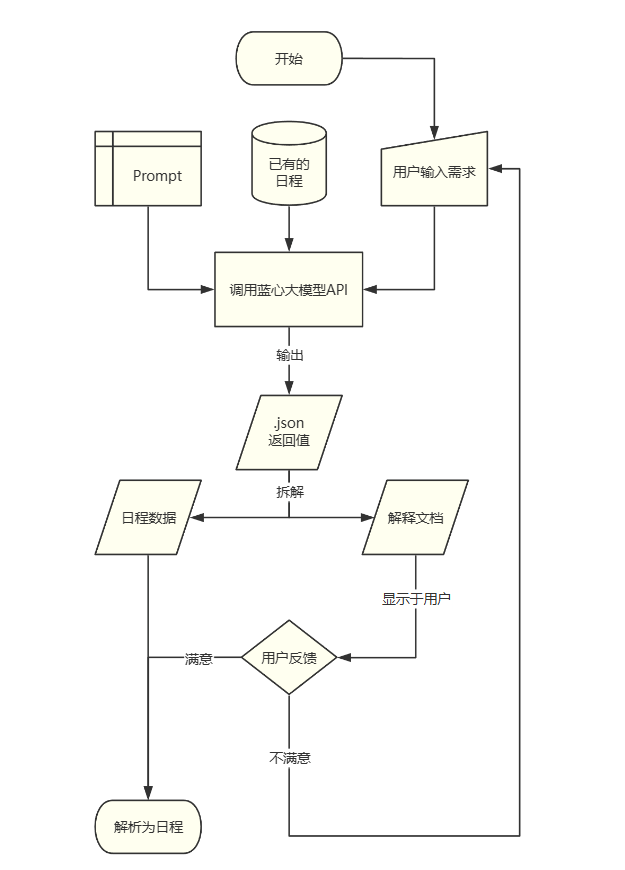
\includegraphics[width=12cm]{figure/flowchart.png}
    \caption{日历应用流程图}
\end{figure}
\end{document}